\section{Explanation (Analysis): What the Cue Explains, and What It Does Not}
\label{sec:explain}

\paragraph{A strong cue is sufficient.}
Where the shortcut is weak the image can still change the decision and its benefit grows with its strength; where the shortcut is reliable enough, visual evidence of any tested strength stops affecting accuracy and the decision is \emph{locked} by the text side.
That a model fine-tuned on a reliable cue comes to rely on it is the expected direction; what the study measures is how the decision and the weakest helpful image change with the cue strength, and that the lock-out strength moves with the benchmark (the veto boundary does not change at thresholds of $+1$ or $+3$ points instead of $+2$, except at $d=0.97$ on A-OKVQA; Supp.~V).
This is a sufficiency result for a planted cue, obtained on two benchmarks and three models of two families (seeds per claim: Supp.~Z), not a statement that natural shortcuts have this effect, nor a universal law.

\paragraph{On the real shortcut the cue is not the only barrier.}
Of the 3{,}000 unseen questions, 235 have a correct option that is \emph{not} the shortest, so the cue cannot decide them.
On these the cue-trained models still gain nothing from the image ($-1.3$ points for Qwen-3B and $0.0$ for Qwen-7B; approximate 95\% intervals $[-4.7,+2.2]$ and $[-2.9,+2.9]$, which exclude $+5$; exploratory, Supp.~X).
A text-only audit (Supp.~Z) shows where the rest comes from: on all 1{,}023 cue-contradicting questions of the benchmark, option-level classifiers that see neither the question nor the image (out-of-fold, folds grouped by near-duplicate component) pick the correct option in $55.0\%$ (95\% interval $[51.8,58.2]$; trained on all questions) and $47.9\%$ $[44.9,51.2]$ (trained on cue-contradicting questions only; chance $25\%$), and the correct option's word overlap with the other options alone gives $43.7\%$ $[40.8,46.9]$, whereas the shortest-option rule gives $0\%$.
The wrong options carry qualifiers (``without'', ``suggesting'', ``only'', ``rather than''): the correct option is the one the distractors resemble.
These are associations in the benchmark's own writing, not a statement about what the models read; together with the null image effect they show that the cue alone does not explain Med-CMR's image-blindness.
Med-CMR's authors state that three language models each generated four distractor candidates and annotators selected four of the twelve under criteria that include visual dependence~\cite{gong2025medcmr}; the resemblance we find is consistent with distractors written as variants of the correct answer, which the data alone cannot confirm.

\begin{figure}[t]
  \centering
  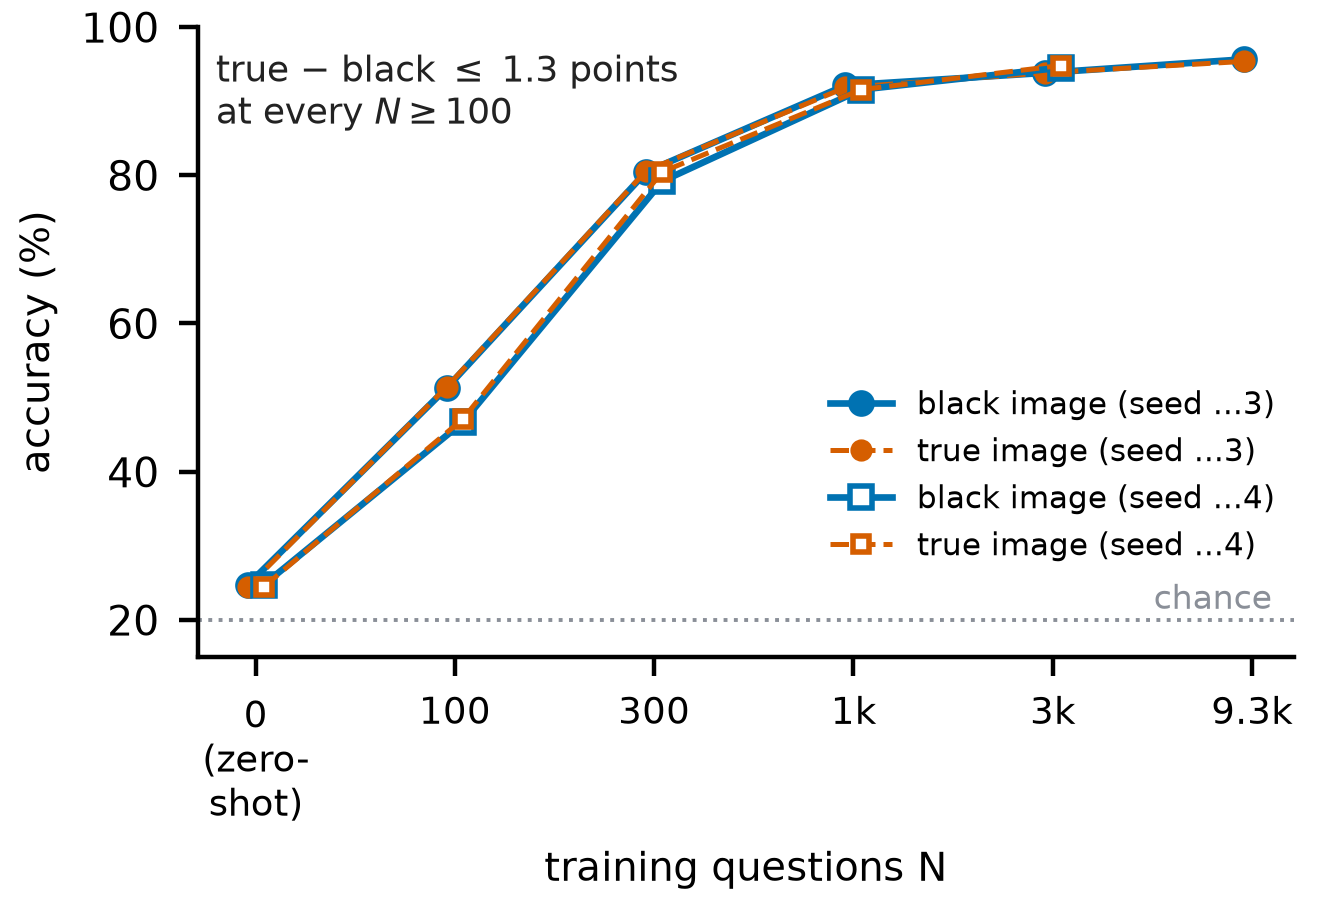
\includegraphics[width=\columnwidth]{fig/f13_curve.png}
  \caption{\textbf{Training on the benchmark installs the shortcut.} Qwen2.5-VL-3B fine-tuned on the first $N$ Med-CMR training questions (A9 recipe, two seeds), accuracy on the 711 held-out questions with a black image (solid) and with the true image (dashed); $N=0$ is zero-shot and 9.3k the full training split (one seed).}
  \label{fig:curve}
\end{figure}

\paragraph{Training on the benchmark installs the shortcut.}
Before fine-tuning, Qwen2.5-VL-3B is at chance on Med-CMR with or without the image ($24.8\%$ with a black image); after 100, 300, 1{,}000 and 9{,}277 training questions it reaches $51\%$, $80\%$, $92\%$ and $95.6\%$ with a black image, and the true-image accuracy tracks it (true minus black at most $1.3$ points at every $N\ge100$; two seeds; all three pre-registered rules held; Fig.~\ref{fig:curve}).
On OmniMedVQA the same comparison at 3B raises the black-image accuracy from $54.0\%$ to $93.2\%$, but on PMC-VQA and A-OKVQA, which have no length cue and low blind ceilings, by only $1.7$ and $0.4$ points (Supp.~Z).
Image-blind accuracy thus has two routes, the benchmark's text artifacts that training on its own split installs (the blind ceiling) and knowledge the model brings (MMMU health: $49.0\%$ without the image against a ceiling of $23.5\%$); the pre-registered 32B tests of the second were not run.
